%package list
\documentclass{article}
\usepackage[top=3cm, bottom=3cm, outer=3cm, inner=3cm]{geometry}
\usepackage{multicol}
\usepackage{graphicx}
\usepackage{url}
%\usepackage{cite}
\usepackage{hyperref}
\usepackage{array}
%\usepackage{multicol}
\newcolumntype{x}[1]{>{\centering\arraybackslash\hspace{0pt}}p{#1}}
\usepackage{natbib}
\usepackage{pdfpages}
\usepackage{multirow}
\usepackage[normalem]{ulem}
\useunder{\uline}{\ul}{}
\usepackage{svg}
\usepackage{xcolor}
\usepackage{listings}
\lstdefinestyle{ascii-tree}{
    literate={├}{|}1 {─}{--}1 {└}{+}1 
  }
\lstset{basicstyle=\ttfamily,
  showstringspaces=false,
  commentstyle=\color{red},
  keywordstyle=\color{blue}
}
%\usepackage{booktabs}
\usepackage{caption}
\usepackage{subcaption}
\usepackage{float}
\usepackage{array}

\newcolumntype{M}[1]{>{\centering\arraybackslash}m{#1}}
\newcolumntype{N}{@{}m{0pt}@{}}


%%%%%%%%%%%%%%%%%%%%%%%%%%%%%%%%%%%%%%%%%%%%%%%%%%%%%%%%%%%%%%%%%%%%%%%%%%%%
%%%%%%%%%%%%%%%%%%%%%%%%%%%%%%%%%%%%%%%%%%%%%%%%%%%%%%%%%%%%%%%%%%%%%%%%%%%%
\newcommand{\itemEmail}{fayamamani@unsa.edu.pe}
\newcommand{\itemStudent}{Francis Willian Ayamamani Añasco}
\newcommand{\itemCourse}{Programación Web 2}
\newcommand{\itemCourseCode}{GUIA-PRLD-001}
\newcommand{\itemSemester}{I}
\newcommand{\itemUniversity}{Universidad Nacional de San Agustín de Arequipa}
\newcommand{\itemFaculty}{Facultad de Ingeniería de Producción y Servicios}
\newcommand{\itemDepartment}{Departamento Académico de Ingeniería de Sistemas e Informática}
\newcommand{\itemSchool}{Escuela Profesional de Ingeniería de Sistemas}
\newcommand{\itemAcademic}{2023 - A}
\newcommand{\itemInput}{Del 5 Junio 2023}
\newcommand{\itemOutput}{Al 5 Junio 2023}
\newcommand{\itemPracticeNumber}{03}
\newcommand{\itemTheme}{Ajax y NodeJS}
%%%%%%%%%%%%%%%%%%%%%%%%%%%%%%%%%%%%%%%%%%%%%%%%%%%%%%%%%%%%%%%%%%%%%%%%%%%%
%%%%%%%%%%%%%%%%%%%%%%%%%%%%%%%%%%%%%%%%%%%%%%%%%%%%%%%%%%%%%%%%%%%%%%%%%%%%

\usepackage[english,spanish]{babel}
\usepackage[utf8]{inputenc}
\AtBeginDocument{\selectlanguage{spanish}}
\renewcommand{\figurename}{Figura}
\renewcommand{\refname}{Referencias}
\renewcommand{\tablename}{Tabla} %esto no funciona cuando se usa babel
\AtBeginDocument{%
	\renewcommand\tablename{Tabla}
}

\usepackage{fancyhdr}
\pagestyle{fancy}
\fancyhf{}
\setlength{\headheight}{30pt}
\renewcommand{\headrulewidth}{1pt}
\renewcommand{\footrulewidth}{1pt}
\fancyhead[L]{\raisebox{-0.2\height}{
\includegraphics[width=3cm]{img/logo_episunsa.png}}}
\fancyhead[C]{\fontsize{7}{7}\selectfont	\itemUniversity \\ \itemFaculty \\ \itemDepartment \\ \itemSchool \\ \textbf{\itemCourse}}
\fancyhead[R]{\raisebox{-0.2\height}{
\includegraphics[width=1.2cm]{img/logo_abet}}}
\fancyfoot[L]{Estudiante Francis Ayamamani Añasco}
\fancyfoot[C]{\itemCourse}
\fancyfoot[R]{Página \thepage}

% para el codigo fuente
\usepackage{listings}
\usepackage{color, colortbl}
\definecolor{dkgreen}{rgb}{0,0.6,0}
\definecolor{gray}{rgb}{0.5,0.5,0.5}
\definecolor{mauve}{rgb}{0.58,0,0.82}
\definecolor{codebackground}{rgb}{0.95, 0.95, 0.92}
\definecolor{tablebackground}{rgb}{0.8, 0, 0}

\lstset{frame=tb,
	language=bash,
	aboveskip=3mm,
	belowskip=3mm,
	showstringspaces=false,
	columns=flexible,
	basicstyle={\small\ttfamily},
	numbers=none,
	numberstyle=\tiny\color{gray},
	keywordstyle=\color{blue},
	commentstyle=\color{dkgreen},
	stringstyle=\color{mauve},
	breaklines=true,
	breakatwhitespace=true,
	tabsize=3,
	backgroundcolor= \color{codebackground},
}

\begin{document}
	
	\vspace*{10px}
	
	\begin{center}	
		\fontsize{17}{17} \textbf{ Informe de Laboratorio \itemPracticeNumber}
	\end{center}
	\centerline{\textbf{\Large Tema: \itemTheme}}
	%\vspace*{0.5cm}	

	\begin{flushright}
		\begin{tabular}{|M{2.5cm}|N|}
			\hline 
			\rowcolor{tablebackground}
			\color{white} \textbf{Nota}  \\
			\hline 
			     \\[30pt]
			\hline 			
		\end{tabular}
	\end{flushright}	

	\begin{table}[H]
		\begin{tabular}{|x{4.7cm}|x{4.8cm}|x{4.8cm}|}
			\hline 
			\rowcolor{tablebackground}
			\color{white} \textbf{Estudiante} & \color{white}\textbf{Escuela}  & \color{white}\textbf{Asignatura}   \\
			\hline 
			{\itemStudent \par \itemEmail} & \itemSchool & {\itemCourse \par Semestre: \itemSemester \par Código: \itemCourseCode}     \\
			\hline 			
		\end{tabular}
	\end{table}		
	
	\begin{table}[H]
		\begin{tabular}{|x{4.7cm}|x{4.8cm}|x{4.8cm}|}
			\hline 
			\rowcolor{tablebackground}
			\color{white}\textbf{Laboratorio} & \color{white}\textbf{Tema}  & \color{white}\textbf{Duración}   \\
			\hline 
			\itemPracticeNumber & \itemTheme & 04 horas   \\
			\hline 
		\end{tabular}
	\end{table}
	
	\begin{table}[H]
		\begin{tabular}{|x{4.7cm}|x{4.8cm}|x{4.8cm}|}
			\hline 
			\rowcolor{tablebackground}
			\color{white}\textbf{Semestre académico} & \color{white}\textbf{Fecha de inicio}  & \color{white}\textbf{Fecha de entrega}   \\
			\hline 
			\itemAcademic & \itemInput &  \itemOutput  \\
			\hline 
		\end{tabular}
	\end{table}
	
	\section{Tarea}
	\begin{itemize}
		\item Para resolver los siguientes ejercicios sólo está permitido usar ciclos, condicionales, definición de listas por comprensión, sublistas, map, join, (+), lambda, zip, append, pop, range.
        \begin{enumerate}
            \item Implemente los métodos de la clase Picture. Se recomienda que implemente la clase picture por etapas, probando realizar los dibujos que se muestran en la siguiente preguntas.
            \item Usando únicamente los métodos de los objetos de la clase Picture dibuje las siguientes figuras (invoque a draw):
            \begin{itemize}
            \item (a)
                \begin{figure}[H]
		          \centering
		          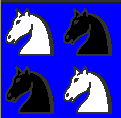
\includegraphics[scale=5,keepaspectratio]{img/ejercicio_02_a.png}
		          %\includesvg{img/automata.svg}
		          %\label{img:mot2}
		          %\caption{Product backlog.}
	            \end{figure}
             \item (b)
                \begin{figure}[H]
		          \centering
		          
\includegraphics[scale=5,keepaspectratio]{img/ejercicio_02_b.png}
		          %\includesvg{img/automata.svg}
		          %\label{img:mot2}
		          %\caption{Product backlog.}
	            \end{figure}
             \item (c)
                \begin{figure}[H]
		          \centering
		          
\includegraphics[scale=5,keepaspectratio]{img/ejercicio_02_c.png}
		          %\includesvg{img/automata.svg}
		          %\label{img:mot2}
		          %\caption{Product backlog.}
	            \end{figure}
             \item (d)
                \begin{figure}[H]
		          \centering
		          
\includegraphics[scale=3.5,keepaspectratio]{img/ejercicio_02_d.png}
		          %\includesvg{img/automata.svg}
		          %\label{img:mot2}
		          %\caption{Product backlog.}
	            \end{figure}
             \item (e)
                \begin{figure}[H]
		          \centering
		          
\includegraphics[scale=3.5,keepaspectratio]{img/ejercicio_02_e.png}
		          %\includesvg{img/automata.svg}
		          %\label{img:mot2}
		          %\caption{Product backlog.}
	            \end{figure}
             \item (f)
                \begin{figure}[H]
		          \centering
		          
\includegraphics[scale=3.5,keepaspectratio]{img/ejercicio_02_f.png}
		          %\includesvg{img/automata.svg}
		          %\label{img:mot2}
		          %\caption{Product backlog.}
	            \end{figure}
             \item (g)
                \begin{figure}[H]
		          \centering
		          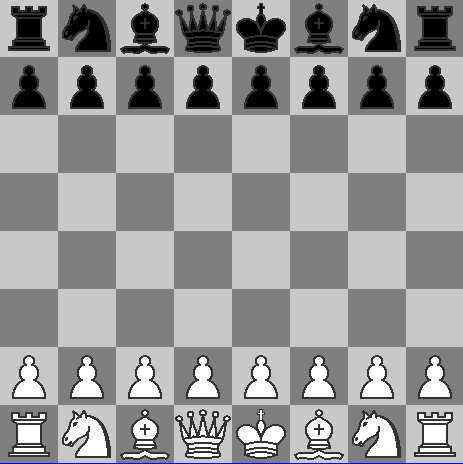
\includegraphics[scale=3.5,keepaspectratio]{img/ejercicio_02_g.png}
		          %\includesvg{img/automata.svg}
		          %\label{img:mot2}
		          %\caption{Product backlog.}
	            \end{figure}
            \end{itemize}
        \end{enumerate}
	\section{MARCO CONCEPTUAL}
	\begin{itemize}
		\item Editor Vim
        \begin{itemize}
            \item Vim es un editor de texto muy eficiente para programar en consola que no tiene nada que envidiar a los editores gráficos.
        \end{itemize}
        \item Instalar Vim en
        \begin{itemize}
            \item GNU/Linux
            \begin{itemize}
                \begin{lstlisting}
                    apt-get install vim
                \end{lstlisting}
            \end{itemize}
            \item MS Windows
            \begin{itemize}
                \item Para descarga en sistemas MS Windows \url{https://www.vim.org/download.php}
            \end{itemize}
            \item MacOS
            \begin{itemize}
                \begin{lstlisting}
                    brew install macvim
                \end{lstlisting}
            \end{itemize}
        \end{itemize}
        \item Git
        \begin{itemize}
            \item Git es un sistema de control de versiones creado por Linus Torvalds. Es eficiente, confiable.
        \end{itemize}
        \item Instalar Git
        \begin{itemize}
            \item GNU/Linux
            \begin{itemize}
                \begin{lstlisting}
                apt-get install git    
                \end{lstlisting}
            \end{itemize}
            \item MS Windows
            \begin{itemize}
                \item Para descarga en sistemas MS Windows \url{https://git-scm.com/download/win}
            \end{itemize}
            \item MacOS
            \begin{itemize}
                \item Para descarga en sistemas MacOS \url{https://git-scm.com/download/mac}
                \begin{lstlisting}
                    brew install git
                \end{lstlisting}
            \end{itemize}
        \end{itemize}
        \item python
        \begin{itemize}
            \item Para un instalación local en sistemas operativos MS Windows utilice: https://www.python.org/downloads/windows/
            \item Tambien ud puede probar código en herramientas online: \url{https://www.programiz.com/python-programming/online-compiler/}
            \item Python en Debian GNU/Linux:
            \begin{itemize}
            \begin{lstlisting}[language=bash,caption={Debian Linux viene con Python 3 y Python 2 preinstalados.}][H]
		          python3 --version
                    Python 3.9.2
	        \end{lstlisting}
            \begin{lstlisting}[language=bash,caption={Instalemos pip, una herramienta que instalará y administrará los paquetes de programación que queramos usar en nuestros proyectos de desarrollo.}][H]
		          sudo apt-get install -y python3-pip
	        \end{lstlisting}
            \begin{lstlisting}[language=bash,caption={Paquetes y herramientas de desarrollo más para instalar para garantizar que tengamos una configuración sólida para nuestro entorno de programación:}][H]
		          sudo apt-get install build-essential libssl-dev libffi-dev python3-dev
	        \end{lstlisting}
            \end{itemize}
            \item Configurar un entorno virtual:
            \begin{itemize}
                \item Los entornos virtuales permiten tener un espacio aislado en los proyectos Python
                \item Garantizando que cada proyecto pueda tener su propio conjunto de dependencias que no interrumpirán a otros proyectos.
                \item Manejando diferentes versiones de los paquetes. Esto es especialmente importante cuando se trabaja con paquetes de terceros.
                \item Puede varios entornos de programación.
                \item Cada entorno es un directorio en la que se ubicaran sus scripts.
                \item Usaremos el módulo venv , que es parte de la biblioteca estándar de Python.
                \begin{lstlisting}[language=bash,caption={Entorno de Linux-Instalemos venv escribiendo:}][H]
    		          sudo apt install -y python3-venv
    	        \end{lstlisting}
                \begin{lstlisting}[language=bash,caption={Entorno de Linux-Para crear un ambiente elija en qué directorio.}][H]
    		          mkdir -p ~/unsa/pw2/labs/lab04/entorno
                        cd ~/unsa/pw2/labs/lab04/entorno
    	        \end{lstlisting}
                \begin{lstlisting}[language=bash,caption={Entorno de Linux-En el directorio crea un entorno virtual ejecutando el siguiente comando:}][H]
    		          virtualenv -p python3 .
    	        \end{lstlisting}
                \begin{lstlisting}[language=bash,caption={Entorno de Linux-Ejecute el script de activación para activar el entorno virtual:}][H]
    		          source ../bin/activate
    	        \end{lstlisting}
            \end{itemize}
        \end{itemize}
	\end{itemize}
	
	\section{URL de Repositorio Github}
	\begin{itemize}
		\item URL del Repositorio GitHub para clonar o recuperar.
		\item \url{https://github.com/rescobedoq/pw2/tree/main/labs/lab04/Tarea-del-Ajedrez}
		\item URL para el laboratorio 04 en el Repositorio GitHub.
		\item \url{https://github.com/rescobedoq/pw2/tree/main/labs/lab04}
	\end{itemize}
	
	\section{Resolucion de la tarea}
	
	\subsection{Explicacion del Codigo}
    \begin{lstlisting}[language=python,caption={Clase Picture}][H]
        from colors import *
        class Picture:
          def __init__(self, img):
            self.img = img;
        
          def __eq__(self, other):
            return self.img == other.img
        
          def _invColor(self, color):
            if color not in inverter:
              return color
            return inverter[color]
        
          def verticalMirror(self):
            """ Devuelve el espejo vertical de la imagen """
            vertical = []
            for value in self.img:
            	vertical.append(value[::-1])
            return vertical
        
          def horizontalMirror(self):
            """ Devuelve el espejo horizontal de la imagen """
            horizontal=self.img[::-1]
            return Picture(horizontal)
        
          def negative(self):
            """ Devuelve un negativo de la imagen """
            neg=[]
            for linea in range(len(self.img)):
                negativo=""
                for pixel in range(len(self.img[linea])):
                    negativo+=self._invColor(self.img[linea][pixel])
                neg.append(negativo)
            return Picture(neg)
        
          def join(self, p):
            """ Devuelve una nueva figura poniendo la figura del argumento 
                al lado derecho de la figura actual """
            nuevo=[]
            for linea in range(len(p.img)):
                nuevo.append(self.img[linea]+p.img[linea])
            return Picture(nuevo)
        
          def up(self, p):
            nuevo=p.img+self.img
            return Picture(nuevo)
        
          def under(self, p):
            """ Devuelve una nueva figura poniendo la figura p sobre la
                figura actual """
            new=[]
            for (linea1,linea2) in zip(range(len(p.img)),range(len(self.img))):
                lineas=""
                for (pixel1,pixel2) in zip(p.img[linea1],self.img[linea2]):
                    if pixel1==" ":
                        lineas+=pixel2
                    else:
                        lineas+=pixel1
                new.append(lineas)
            return Picture(new)
          
          def horizontalRepeat(self, n):
            """ Devuelve una nueva figura repitiendo la figura actual al costado
                la cantidad de veces que indique el valor de n """
            repeticion=[]
            for lineas in range(len(self.img)):
                repeticion.append(self.img[lineas]*int(n))
            return Picture(repeticion)
        
          def verticalRepeat(self, n):
            repeticion=[]
            repeticion+=self.img*int(n)
            return Picture(repeticion)
    \end{lstlisting}
	\begin{itemize}
	    \item la funcion \textbf{verticalMirror}; comienza creando una variable Lista (\textbf{vertical}), para luego con una estructura de dato repetitiva (for), recorre cada linea de objeto self.img; que es nuestro elemento local; para luego cambiar el orden de los elementos de esta linea [ primero = final]. Finalmente agrega esta linea a la Lista antes creada, mediante el metodo \textbf{append()}.
        \item la funcion \textbf{horizontalMirror}; comienza creando una variable Lista (\textbf{horizontal}), para luego cambiar el orden de las lineas de \textbf{self.img} [ primero = final]. Finalmente se le asigna estos cambios de la variable .img a horizontal.
        \item la funcion \textbf{negative}; comienza creando una variable Lista (\textbf{neg}), para luego recorrer las lineas de la ficha, luego de ello dentro de este recorrido se crea una variable local, que guarde la nueva linea negativa. Y para ello, hacemos un for anidado, que recorra cada pixel o en este caso cada elemento de la cadena, para luego cambiarla por su negativo, segun el diccionario.
        \item la funcion \textbf{join}; comienza creando una variable Lista (\textbf{nuevo}), para luego concatenar los contenidos de cada linea i de \textbf{self.img} y \textbf{p.img}; mediante el bucle for.
        \item la funcion \textbf{under}; comienza creando una variable Lista (\textbf{new}), para luego cambiar los pixeles ( caracteres de la cadena de texto ), mediante una estructura if que verifica si el pixel esta vacio, entonces lo remplaza con el pixel de self.img; pero si no entonces introduce el pixel de p.img
        \item la funcion \textbf{up}; comienza creando una variable Lista (\textbf{nuevo}), para luego concatenar las listas:
        \begin{lstlisting}[language=python,caption={Codigo de ejemplo}][H]
            lista1=[1,2,3]
            lista2=[5,6,7]
            lista3= lista1+lista2
            print (lista3)
        \end{lstlisting}
        \begin{lstlisting}[language=python,caption={Resultado de Consola}][H]
            [1,2,3,4,5,6,7]
        \end{lstlisting}
        \item la funcion \textbf{horizontalRepeat}; utiliza la misma logica que el algoritmo de \textbf{horizontalMirror}, agregando el simbolo \textbf{*} para poder repetir una linea:
        \begin{lstlisting}[language=python,caption={Codigo de ejemplo}][H]
            comentario="Hola pepe"
            print (comentario*int(2))
        \end{lstlisting}
        \begin{lstlisting}[language=python,caption={Resultado de Consola}][H]
            Hola pepeHola pepe
        \end{lstlisting}
        \item la funcion \textbf{verticalRepeat}; al igual que \textbf{horizontalRepeat}, utiliza la simbolo de \textbf{*}
	\end{itemize}
    \section{Commit-Estructura}
    \subsection{Commit-Laboratorio 04}
    \subsubsection{Lista en GITHUB}
                \begin{figure}[H]
		          \centering
		          
\includegraphics[scale=0.4,keepaspectratio]{img/HoriMirror.png}
		          %\includesvg{img/automata.svg}
		          %\label{img:mot2}
		          %\caption{Product backlog.}
	            \end{figure}
                \begin{figure}[H]
		          \centering
		          
\includegraphics[scale=0.4,keepaspectratio]{img/Negative.png}
		          %\includesvg{img/automata.svg}
		          %\label{img:mot2}
		          %\caption{Product backlog.}
	            \end{figure}
                \begin{figure}[H]
		          \centering
		          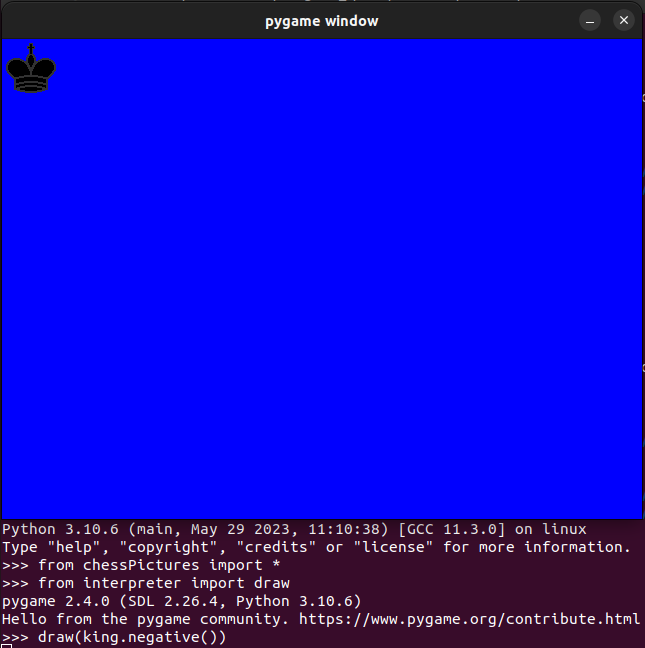
\includegraphics[scale=0.4,keepaspectratio]{img/PruebaNegative.png}
		          %\includesvg{img/automata.svg}
		          %\label{img:mot2}
		          %\caption{Product backlog.}
	            \end{figure}
                \begin{figure}[H]
		          \centering
		          
\includegraphics[scale=0.4,keepaspectratio]{img/Join.png}
		          %\includesvg{img/automata.svg}
		          %\label{img:mot2}
		          %\caption{Product backlog.}
	            \end{figure}
                \begin{figure}[H]
		          \centering
		          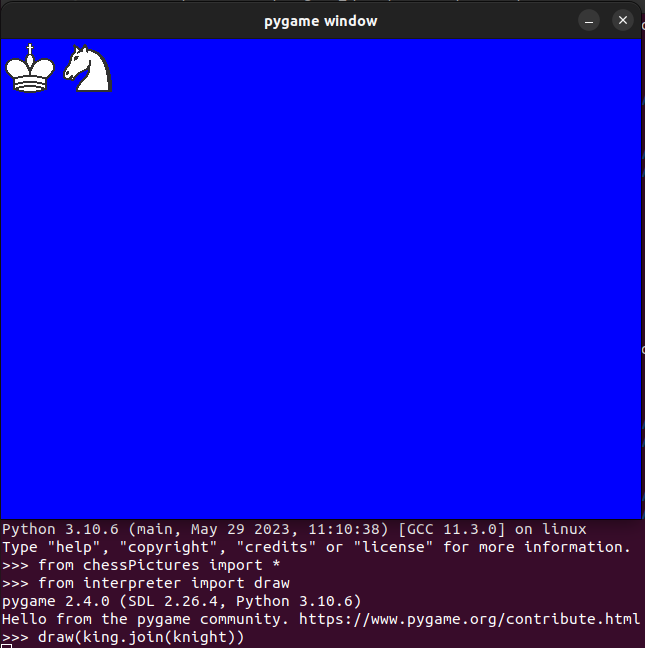
\includegraphics[scale=0.4,keepaspectratio]{img/PruebaJoin.png}
		          %\includesvg{img/automata.svg}
		          %\label{img:mot2}
		          %\caption{Product backlog.}
	            \end{figure}
                \begin{figure}[H]
		          \centering
		          
\includegraphics[scale=0.4,keepaspectratio]{img/Up.png}
		          %\includesvg{img/automata.svg}
		          %\label{img:mot2}
		          %\caption{Product backlog.}
	            \end{figure}
                \begin{figure}[H]
		          \centering
		          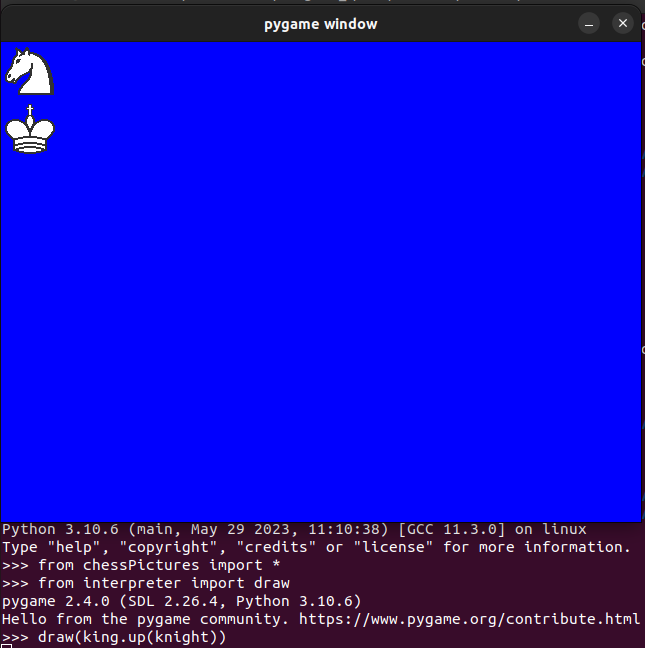
\includegraphics[scale=0.4,keepaspectratio]{img/PruebaUp.png}
		          %\includesvg{img/automata.svg}
		          %\label{img:mot2}
		          %\caption{Product backlog.}
	            \end{figure}
                \begin{figure}[H]
		          \centering
		          
\includegraphics[scale=0.4,keepaspectratio]{img/horizontRepeat.png}
		          %\includesvg{img/automata.svg}
		          %\label{img:mot2}
		          %\caption{Product backlog.}
	            \end{figure}
                \begin{figure}[H]
		          \centering
		          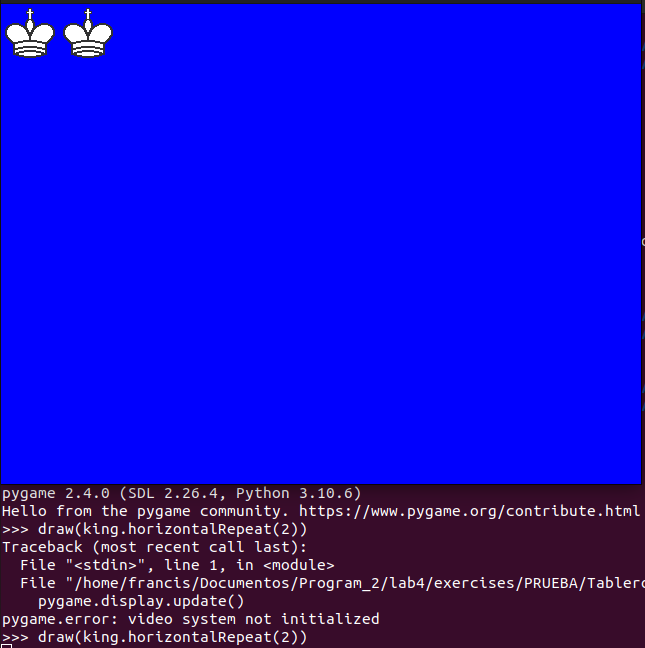
\includegraphics[scale=0.4,keepaspectratio]{img/PruebahorizontalRepeat.png}
		          %\includesvg{img/automata.svg}
		          %\label{img:mot2}
		          %\caption{Product backlog.}
	            \end{figure}
                \begin{figure}[H]
		          \centering
		          
\includegraphics[scale=0.4,keepaspectratio]{img/Under.png}
		          %\includesvg{img/automata.svg}
		          %\label{img:mot2}
		          %\caption{Product backlog.}
	            \end{figure}
                \begin{figure}[H]
		          \centering
		          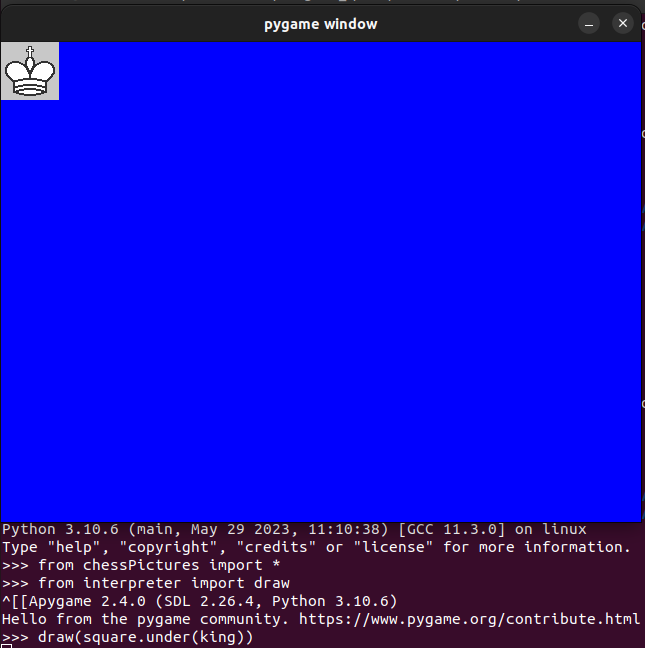
\includegraphics[scale=0.4,keepaspectratio]{img/PruebaUnder.png}
		          %\includesvg{img/automata.svg}
		          %\label{img:mot2}
		          %\caption{Product backlog.}
	            \end{figure}
                \begin{figure}[H]
		          \centering
		          
\includegraphics[scale=0.4,keepaspectratio]{img/EjA.png}
		          %\includesvg{img/automata.svg}
		          %\label{img:mot2}
		          %\caption{Product backlog.}
	            \end{figure}
                \begin{figure}[H]
		          \centering
		          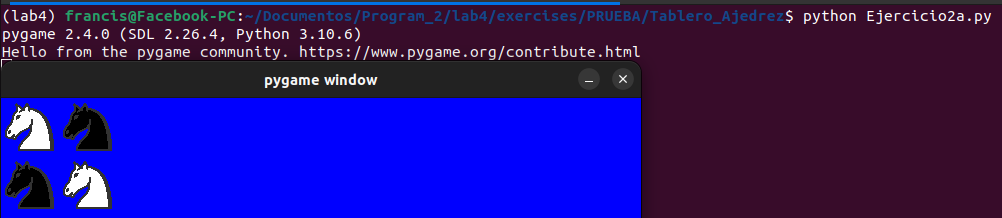
\includegraphics[scale=0.4,keepaspectratio]{img/ResultadoA.png}
		          %\includesvg{img/automata.svg}
		          %\label{img:mot2}
		          %\caption{Product backlog.}
	            \end{figure}
                \begin{figure}[H]
		          \centering
		          
\includegraphics[scale=0.4,keepaspectratio]{img/EjB.png}
		          %\includesvg{img/automata.svg}
		          %\label{img:mot2}
		          %\caption{Product backlog.}
	            \end{figure}
                \begin{figure}[H]
		          \centering
		          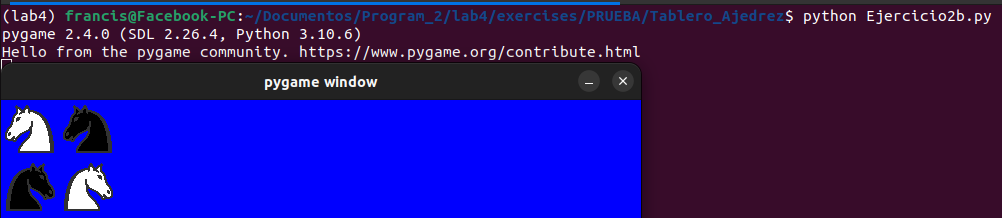
\includegraphics[scale=0.4,keepaspectratio]{img/ResultadoB.png}
		          %\includesvg{img/automata.svg}
		          %\label{img:mot2}
		          %\caption{Product backlog.}
	            \end{figure}
                \begin{figure}[H]
		          \centering
		          
\includegraphics[scale=0.4,keepaspectratio]{img/EjC.png}
		          %\includesvg{img/automata.svg}
		          %\label{img:mot2}
		          %\caption{Product backlog.}
	            \end{figure}
                \begin{figure}[H]
		          \centering
		          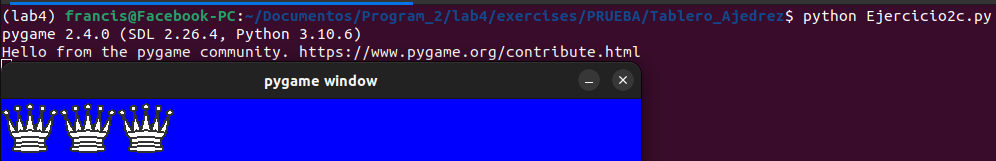
\includegraphics[scale=0.4,keepaspectratio]{img/ResultadoC.png}
		          %\includesvg{img/automata.svg}
		          %\label{img:mot2}
		          %\caption{Product backlog.}
	            \end{figure}
                \begin{figure}[H]
		          \centering
		          
\includegraphics[scale=0.4,keepaspectratio]{img/EjD.png}
		          %\includesvg{img/automata.svg}
		          %\label{img:mot2}
		          %\caption{Product backlog.}
	            \end{figure}
                \begin{figure}[H]
		          \centering
		          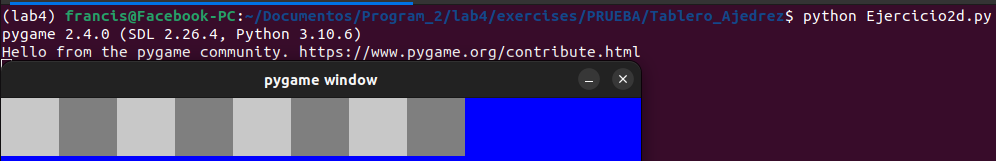
\includegraphics[scale=0.4,keepaspectratio]{img/ResultadoD.png}
		          %\includesvg{img/automata.svg}
		          %\label{img:mot2}
		          %\caption{Product backlog.}
	            \end{figure}
                \begin{figure}[H]
		          \centering
		          
\includegraphics[scale=0.4,keepaspectratio]{img/EjE.png}
		          %\includesvg{img/automata.svg}
		          %\label{img:mot2}
		          %\caption{Product backlog.}
	            \end{figure}
                \begin{figure}[H]
		          \centering
		          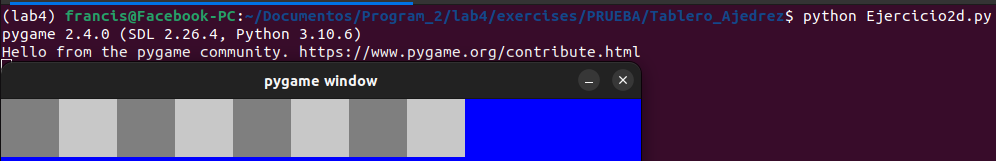
\includegraphics[scale=0.4,keepaspectratio]{img/ResultadoE.png}
		          %\includesvg{img/automata.svg}
		          %\label{img:mot2}
		          %\caption{Product backlog.}
	            \end{figure}
                \begin{figure}[H]
		          \centering
		          
\includegraphics[scale=0.4,keepaspectratio]{img/EjF.png}
		          %\includesvg{img/automata.svg}
		          %\label{img:mot2}
		          %\caption{Product backlog.}
	            \end{figure}
                \begin{figure}[H]
		          \centering
		          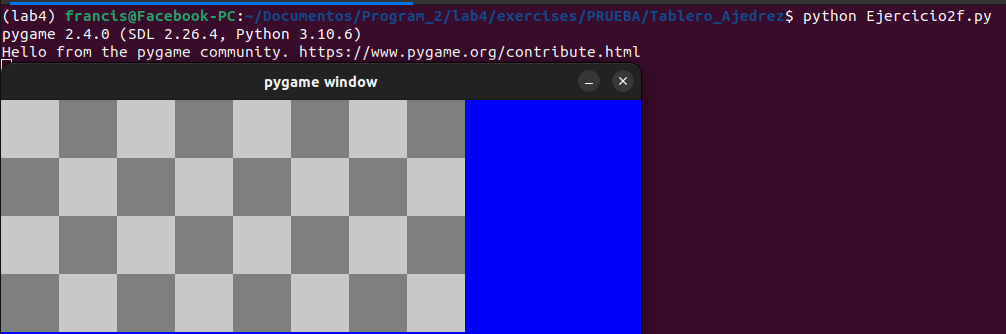
\includegraphics[scale=0.4,keepaspectratio]{img/ResultadoF.png}
		          %\includesvg{img/automata.svg}
		          %\label{img:mot2}
		          %\caption{Product backlog.}
	            \end{figure}
                \begin{figure}[H]
		          \centering
		          
\includegraphics[scale=0.4,keepaspectratio]{img/EjG.png}
		          %\includesvg{img/automata.svg}
		          %\label{img:mot2}
		          %\caption{Product backlog.}
	            \end{figure}
                \begin{figure}[H]
		          \centering
		          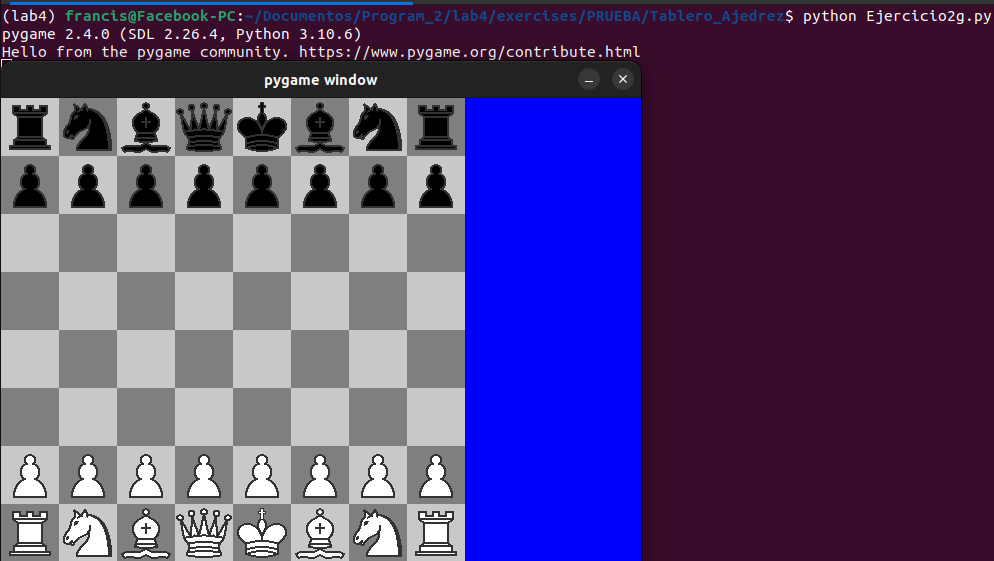
\includegraphics[scale=0.4,keepaspectratio]{img/ResultadoG.png}
		          %\includesvg{img/automata.svg}
		          %\label{img:mot2}
		          %\caption{Product backlog.}
	            \end{figure}
	\subsection{Estructura de laboratorio 04}
	\begin{itemize}	
		\item El contenido que se entrega en este laboratorio es el siguiente:
	\end{itemize}
\begin{lstlisting}[style=ascii-tree]
lab4/
|--- exercises/
    |   |--- esEscalar.py
    |   |--- esUnitaria.py
    |   |--- prueba.py
    |   |--- PRUEBA
            |--- Tablero_Ajedrez
            |   |--- .gitignore
            |   |--- Ejercicio2a.py
            |   |--- Ejercicio2b.py
            |   |--- Ejercicio2c.py
            |   |--- Ejercicio2d.py
            |   |--- Ejercicio2f.py
            |   |--- Ejercicio2e.py
            |   |--- Ejercicio2f.py
            |   |--- Ejercicio2g.py
            |   |--- chessPictures.py
            |   |--- colors.py
            |   |--- interpreter.py
            |   |--- picture.py
            |   |--- pieces.py
            |--- chessMain.py  
            |--- chessEngi.py
            |--- chessPicture
            |   |--- nA.png
            |   |--- nC.png
            |   |--- nk.png
            |   |--- nP.png
            |   |--- nR.png
            |   |--- nT.png
            |   |--- piotr-makowski-27LH_0jXKYI-unsplash.jpg
            |   |--- wA.png
            |   |--- wC.png
            |   |--- wk.png
            |   |--- wP.png
            |   |--- wR.png
            |   |--- wT.png   
\end{lstlisting}    

\section{Cuestionario}
	\begin{itemize}
		\item ¿Qué son los archivos *.pyc?
        \\ Los archivos .pyc son archivos de código fuente compilado en el lenguaje de programación Python. Cuando se ejecuta un programa Python, el intérprete de Python compila el código fuente a un código de bytes intermedio llamado "bytecode". Estos archivos .pyc contienen el bytecode compilado, que es una representación más eficiente y rápida del código fuente original.
        \item ¿Para qué sirve el directorio pycache?
        \\ Cuando se ejecuta un programa Python, el intérprete busca un archivo .pyc correspondiente al archivo .py que se está ejecutando. Si no encuentra el archivo .pyc o si el archivo .pyc existente está desactualizado, el intérprete compila el código fuente y genera un nuevo archivo .pyc. Este archivo .pyc se guarda en el directorio pycache junto con una estructura de carpetas que refleja la ubicación relativa del archivo .py original.
        \item ¿Cuáles son los usos y lo que representa el subguión en Python?
        \\En Python, el subguión se utiliza a menudo en la importación parcial de módulos o paquetes,a veces, ademas se utiliza como una variable especial que representa el resultado del cálculo anterior. Esto permite acceder al resultado anterior sin necesidad de asignarlo a una variable explícitamente.
        
	\end{itemize}		

	\section{\textcolor{red}{Rúbricas}}
	
	\subsection{\textcolor{red}{Entregable Informe}}
	\begin{table}[H]
		\caption{Tipo de Informe}
		\setlength{\tabcolsep}{0.5em} % for the horizontal padding
		{\renewcommand{\arraystretch}{1.5}% for the vertical padding
		\begin{tabular}{|p{3cm}|p{12cm}|}
			\hline
			\multicolumn{2}{|c|}{\textbf{\textcolor{red}{Informe}}}  \\
			\hline 
			\textbf{\textcolor{red}{Latex}} & \textcolor{blue}{El informe está en formato PDF desde Latex,  con un formato limpio (buena presentación) y facil de leer.}   \\ 
			\hline 
			
			
		\end{tabular}
	}
	\end{table}
	
	\clearpage
	
	\subsection{\textcolor{red}{Rúbrica para el contenido del Informe y demostración}}
	\begin{itemize}			
		\item El alumno debe marcar o dejar en blanco en celdas de la columna \textbf{Checklist} si cumplio con el ítem correspondiente.
		\item Si un alumno supera la fecha de entrega,  su calificación será sobre la nota mínima aprobada, siempre y cuando cumpla con todos lo items.
		\item El alumno debe autocalificarse en la columna \textbf{Estudiante} de acuerdo a la siguiente tabla:
	
		\begin{table}[ht]
			\caption{Niveles de desempeño}
			\begin{center}
			\begin{tabular}{ccccc}
    			\hline
    			 & \multicolumn{4}{c}{Nivel}\\
    			\cline{1-5}
    			\textbf{Puntos} & Insatisfactorio 25\%& En Proceso 50\% & Satisfactorio 75\% & Sobresaliente 100\%\\
    			\textbf{2.0}&0.5&1.0&1.5&2.0\\
    			\textbf{4.0}&1.0&2.0&3.0&4.0\\
    		\hline
			\end{tabular}
		\end{center}
	\end{table}	
	
	\end{itemize}
	
	\begin{table}[H]
		\caption{Rúbrica para contenido del Informe y demostración}
		\setlength{\tabcolsep}{0.5em} % for the horizontal padding
		{\renewcommand{\arraystretch}{1.5}% for the vertical padding
		%\begin{center}
		\begin{tabular}{|p{2.7cm}|p{7cm}|x{1.3cm}|p{1.2cm}|p{1.5cm}|p{1.1cm}|}
			\hline
    		\multicolumn{2}{|c|}{Contenido y demostración} & Puntos & Checklist & Estudiante & Profesor\\
			\hline
			\textbf{1. GitHub} & Hay enlace URL activo del directorio para el  laboratorio hacia su repositorio GitHub con código fuente terminado y fácil de revisar. &2 &X &2 & \\ 
			\hline
			\textbf{2. Commits} &  Hay capturas de pantalla de los commits más importantes con sus explicaciones detalladas. (El profesor puede preguntar para refrendar calificación). &4 &X &2 & \\ 
			\hline 
			\textbf{3. Código fuente} &  Hay porciones de código fuente importantes con numeración y explicaciones detalladas de sus funciones. &2 &X &1 & \\ 
			\hline 
			\textbf{4. Ejecución} & Se incluyen ejecuciones/pruebas del código fuente  explicadas gradualmente. &2 &X &1 & \\ 
			\hline			
			\textbf{5. Pregunta} & Se responde con completitud a la pregunta formulada en la tarea.  (El profesor puede preguntar para refrendar calificación).  &2 &X &2 & \\ 
			\hline	
			\textbf{6. Fechas} & Las fechas de modificación del código fuente estan dentro de los plazos de fecha de entrega establecidos. &2 &X &1 & \\ 
			\hline 
			\textbf{7. Ortografía} & El documento no muestra errores ortográficos. &2 &X &2 & \\ 
			\hline 
			\textbf{8. Madurez} & El Informe muestra de manera general una evolución de la madurez del código fuente,  explicaciones puntuales pero precisas y un acabado impecable.   (El profesor puede preguntar para refrendar calificación).  &4 &X &1 & \\ 
			\hline
			\multicolumn{2}{|c|}{\textbf{Total}} &20 & &12 & \\ 
			\hline
		\end{tabular}
		%\end{center}
		%\label{tab:multicol}
		}
	\end{table}
	
\clearpage

\section{Referencias}
\begin{itemize}			
	\item \url{https://www.w3schools.com/java/default.asp}
	\item \url{https://www.geeksforgeeks.org/insertion-sort/}
    \item \url{https://github.com/WillianAyamamani/pw2-lab-d-23a/tree/main/lab1}
\end{itemize}	
	
%\clearpage
%\bibliographystyle{apalike}
%\bibliographystyle{IEEEtranN}
%\bibliography{bibliography}
			
\end{document}